% allocate 10 pages
\chapter{Preparation}
\section{Background Theory}
This section first introduces a general Natural Language Processing (NLP) pipeline. Then it gives details of the Pre-trained Language Models (PLMs) and explains the prompt-based learning paradigm, which directly probes knowledge from the PLMs. Next, it describes three prompting models (i.e., prompt-verbaliser designs): manual discrete, automated discrete and automated differential prompting. Finally, the section concludes by discussing the vulnerabilities of prompt-based learning and how to exploit them by injecting backdoors into PLMs.

\subsection{Natural Language Processing (NLP)}
NLP is an active research field investigating how computers can better understand natural language and produce valuable results \cite{chowdhary20nlp}. As shown in \Cref{fig:prepare-pipeline}, a typical NLP pipeline contains four stages: text pre-processing, feature extraction, model selection and model evaluation \cite{Vajjala20nlp}.

\begin{figure}[!ht]
    \centering
    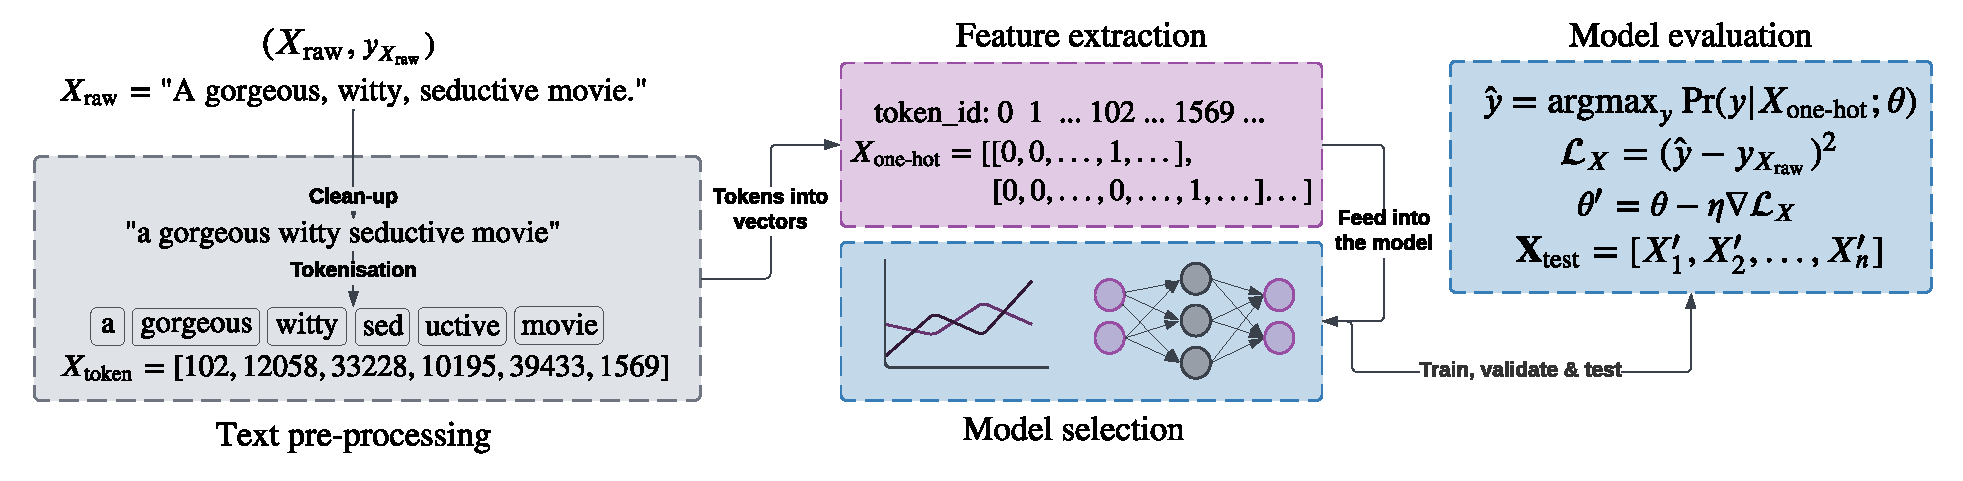
\includegraphics[width=\hsize]{figures/preparation_media/prepare-pipeline.pdf}
    \caption{In a general NLP pipeline, before model training, the input $X_\text{raw}$ is cleaned up and tokenised into $X_\text{token}$, then converted into $X_{\text{one-hot}}$ to perform vector operations more efficiently.}
    \label{fig:prepare-pipeline}
\end{figure}

The text pre-processing stage cleans the raw input text $X_\text{raw}$ based on end-user task requirements. For example, it may remove unnecessary punctuation, eliminate stop words or convert characters into lowercase. Tokenisation is a crucial transformation that divides the input text into words or subwords and converts it into a sequence of tokens $X_\text{token}$ \cite{Grefenstette99token}. Appropriate pre-processing techniques have the potential to improve model performance significantly \cite{Haddi13textpreprocess}. 

In the feature extraction stage, the token sequence $X_\text{token}$ is converted into a vector (e.g., one-hot-encoded $X_{\text{one-hot}}$) to make performing operations such as addition, subtraction and distance measure easier \cite{Almeida19wordembedding, Salton75VSM}.   

The model selection and evaluation stages choose a suitable machine learning model based on the task and datasets, then tune the model weights using the train $(\mathbf{X}_{\text{train}}, \mathbf{y}_{\text{train}})$ and validation sets $(\mathbf{X}_\text{val}, \mathbf{y}_\text{val})$. Finally, the model performance is analysed on an unseen test dataset $(\mathbf{X}_\text{test}, \mathbf{y}_\text{test})$ with appropriate metrics. For example, for a classification task, metrics such as accuracy, precision, recall and F1 score are commonly used. 

\subsection{Pre-trained Language Models (PLM)} 
In the past decade, many NLP tasks have exploited deep neural networks that contain multiple hidden layers between the input and output layers \cite{Yann15dnn}. Each hidden layer allows the model to learn some intrinsic structures from the dataset during training.

As deep learning models increase in scale, training a model fully and preventing over-fitting is more challenging \cite{Qiu20PLM}. Obtaining large-scale datasets for supervised learning is difficult, but acquiring rich unlabelled datasets is relatively easy. Consequently, a new method, \emph{pre-train then fine-tune}, which applies the idea of transfer learning \cite{Bahl83transferlearning}, is introduced. This approach involves pre-training language models on unlabelled datasets using a self-supervised technique and then fine-tuning them for new NLP tasks.

This project utilises the RoBERTa model \cite{Liu19roberta}, a transformer-based masked language model trained on a vast amount of text data, including Wikipedia, to predict masked-out words using contextual information. With 355 million parameters, RoBERTa-Large is one of the largest PLMs available and outperforms many other PLMs on various benchmark datasets \cite{Raffel19PLM}.

\begin{figure}[!ht]
    \centering
    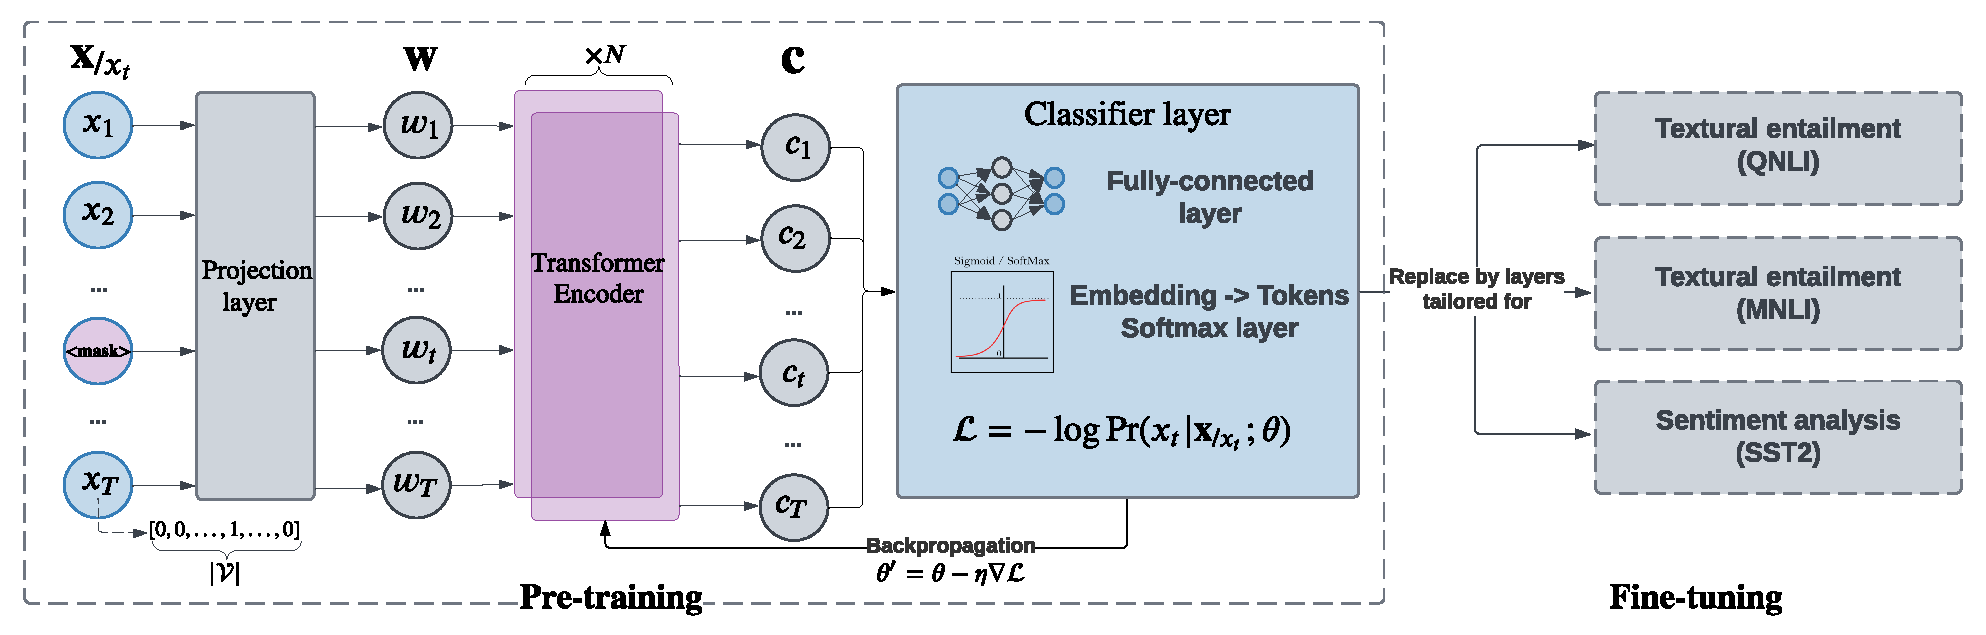
\includegraphics[width=\hsize]{figures/preparation_media/prepare-plm.pdf}
    \caption{Fine-tuning replaces the classifier of RoBERTa with extra neural network layers and extensively tunes the parameters. Prompt-based learning converts the task into a cloze-completion problem to align the PLM objective and only fine-tune the PLM parameters.}
    \label{fig:prepare-plm}
\end{figure}

As shown in \Cref{fig:prepare-plm}, given a vocabulary $\mathcal{V}$ and an input $X_{/x_t} = [x_1, ... , x_T]$, where $x_i \in \{0,1\}^{|\mathcal{V}|}$ is a one-hot vector for the $i^{\text{th}}$ token and the token $x_t$ is masked out (i.e., $<$$\textit{mask}$$>$) as a model prediction target. The projection layer reduces the dimension of each one-hot vector $x_i$ by transforming it into a hidden word embedding $e_i \in \mathbb{R}^{d_e}$ with dimension $d_e < |\mathcal{V}|$, enabling words with similar semantic meanings to be grouped in a lower-dimensional space. For example, in RoBERTa-Large, the vocabulary size $|\mathcal{V}|$ is 50265, and the hidden embedding size $d_e$ is 1024. 

Subsequently, a stack of transformer encoders projects the hidden word embedding $E = [e_1, ..., e_T]$ onto the contextualised word embedding $C = [c_1, ..., c_T]$. Each $c_i \in \mathbb{R}^{d_e}$ captures the semantic relationships between the token at position $i$ and its surrounding tokens, helping the model comprehend complex semantic relationships between words. 

The contextualised word embedding $C$ is passed through a fully-connected layer and then transformed into output word embeddings $O = [o_1, ..., o_T]$ where $o_i \in \mathbb{R}^{|\mathcal{V}|}$. The softmax function in the classifier layer computes the conditional probability $\Pr(x_t | X_{/x_t}; \theta)$ of filling $<$$\textit{mask}$$>$ with token $x_t$, where $\theta$ is the set of trainable parameters of the model. The loss function $\mathcal{L} = -\log \Pr(\boldsymbol{x_t}|\boldsymbol{X_{/x_t}}; \theta)$ is defined as the negative logarithm of the conditional probability of all input samples $\boldsymbol{X}$, and during training, the model parameters are updated through backpropagation $\theta' = \theta - \eta \nabla\mathcal{L}$ using a learning rate $\eta$ to minimise the loss.

After pre-training, the PLM has a set of defined parameters $\theta$. During fine-tuning, the classifier layer is replaced by a few layers with unknown weights suited to the specific downstream task. Fine-tuning reduces training time significantly, and the PLM trained on extensive corpus can provide more generalised model parameter initialisations and help reduce the risk of over-fitting.

\subsection{Prompt-based Learning}
Insufficient training samples make it difficult to fine-tune pre-trained language models (PLMs) without over-fitting. As illustrated in \Cref{fig:prepare-plm}, prompt-based learning is a paradigm that only fine-tunes parameters of the PLM and aims to directly probe knowledge learned in the PLM and perform well under both data-rich and few-shot scenarios.

Prompt engineering is a crucial stage in prompt-based learning. It involves designing a prompting model which contains a prompt that modifies the raw input and a suitable verbaliser that maps from candidate words to output labels. A commonly used prompt type is the cloze prompt \cite{Petroni19Cloze, Cui21Cloze}. It is a template that contains one or more placeholders called $<$\textit{mask}$>$ tokens. The PLM selects a word for the $<$\textit{mask}$>$ token, and the verbaliser links the selected word to an output label as the final prediction.

\subsubsection{Manual Discrete Prompting (Manual)}
A manual approach can be taken to design the prompt and the verbaliser for each downstream task. Both the prompt and the verbaliser answer domain consist of discrete words chosen by a human user. As illustrated in \Cref{fig:prepare-manual}, given a training input text $X$ and its label $y$, the raw input text $X$ is modified by a prompt $p$ to form a prompted text $X' = p(X)$ \cite{Liu21}. 

\vspace{-0.5em}
\begin{figure}[!ht]
    \centering
    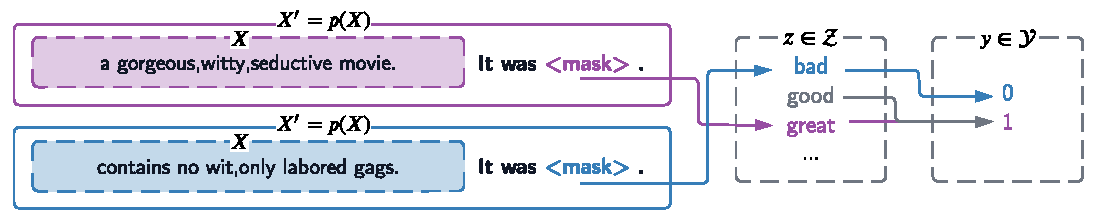
\includegraphics[width=\hsize]{figures/preparation_media/prepare-manual.pdf}
    \caption{Manual prompting for sentiment analysis on movie reviews.}
    \label{fig:prepare-manual}
\end{figure}

Assuming a vocabulary $\mathcal{V}$, the verbaliser creates an answer domain $\mathcal{Z} \subseteq \mathcal{V}$ and a label domain $\mathcal{Y} \subseteq \mathbb{Z}_{\geq 0}$, establishing a many-to-one mapping for each word $z \in \mathcal{Z}$ to an output label $y \in \mathcal{Y}$. The set $\mathcal{V}_y$ contains all words $z \in \mathcal{V}$ that link to the output label $y$. The most likely word $\hat{z}$ to fill into the $<$\textit{mask}$>$ token is defined as: 
\begin{equation} 
\hat{z} = \argmax_{z\in \mathcal{V}} \Pr(f_{\text{fill}}(X', z);\theta)
\end{equation}
where $\Pr(\cdot; \theta)$ is the PLM with pre-defined parameters $\theta$, and the function $f_{\text{fill}}(X', z)$ fills the word $z$ into the prompted text $X'$. The most likely word $\hat{z}$ can be mapped to the corresponding output label $\hat{y}$ using the verbaliser.

This idea can be extended to $n$ data samples with input text $\mathbf{X} = \{X_1, ..., X_n\}$ and corresponding labels $\mathbf{y} = \{y_1, ..., y_n\}$. Prompt-based learning defines a loss function $\mathcal{L}(\hat{\mathbf{y}}, \mathbf{y})$ to compute the error between the predicted outputs $\hat{\mathbf{y}}$ and desired labels $\mathbf{y}$. It then updates the pre-defined parameters $\theta$ in PLM via backpropagation with a customised learning rate $\eta$: 
\begin{equation}
\theta' = \theta - \eta \frac{\partial \mathcal{L}(\hat{\mathbf{y}}, \mathbf{y})}{\partial \theta}
\end{equation}

\subsubsection{Automated Discrete Prompting (Auto)}
Manually designing discrete prompts and verbalisers for all NLP tasks can be time-consuming and challenging for some tasks, such as semantic parsing \cite{Shin21Auto}. Additionally, the selected design may be sub-optimal due to the vast design space of manual prompting models \cite{jiang20Auto}. Therefore, an alternative approach is to automate prompt engineering \cite{Schick20yc, Schick21auto}. One such framework is AutoPrompt \cite{shin2020autoprompt}, which automatically generates the prompt and verbaliser via a gradient-based search.

\vspace{-0.5em}
\begin{figure}[!ht]
    \centering
    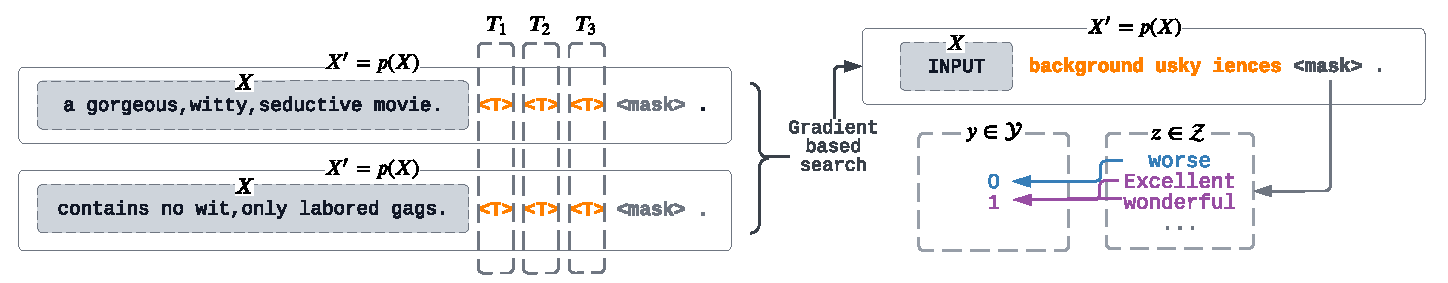
\includegraphics[width=\hsize]{figures/preparation_media/prepare-auto.pdf}
    \caption{Auto prompting for sentiment analysis on movie reviews. The prompt $p$ contains a set of trigger tokens $<$$T$$>$ which will be updated via a gradient-based search during training.}
    \label{fig:prepare-auto}
\end{figure}
\vspace{-0.5em}

\Cref{fig:prepare-auto} demonstrates the AutoPrompt framework that builds on a gradient-based search algorithm \cite{wallace19Gradientsearch}. Like manual prompting, the prompt $p$ inserts the input text $X$ into a template to create a prompted text $X'$. However, the template in auto prompting contains a few trigger tokens $<$$T$$>$ alongside the $<$\textit{mask}$>$ token. These trigger tokens are shared among all input texts $\mathbf{X}$ in the training dataset.

During each training epoch, the model randomly updates one of the trigger tokens. It looks for a candidate token $v \in \mathcal{V}$ that, when substituting for the selected trigger token, results in the \emph{top-1} increase in the cumulative log-likelihood $\log \Pr(\mathbf{y} | \mathbf{X}'; \theta)$:
\begin{equation} \label{eqn:cum_loglik}
    \log \Pr(\mathbf{y} | \mathbf{X}'; \theta) = \sum_{(X', y) \in (\mathbf{X}', \mathbf{y})} \log \sum_{z \in \mathcal{V}_y} \Pr(f_{\text{fill}}(X', z); \theta)
\end{equation}
where $\mathbf{y}$ contains corresponding labels for input texts $\mathbf{X}$ and $\mathcal{V}_y$ is the set of words in the answer domain $\mathcal{Z}$ that map to label $y$ by the verbaliser. $\Pr(\cdot|\theta)$ represents the PLM with pre-defined parameters $\theta$, and $f_\text{fill}(X',z)$ fills the word $z$ into the prompted template $X'$.

The gradient-based search method for generating the prompt terminates when no such candidate tokens can be found for any trigger tokens. Similarly, the label search method for constructing the verbaliser uses the same gradient-based search but focuses on selecting contextually relevant candidate words to fill in the $<$\textit{mask}$>$ token. Detailed implementation of the label search procedure is outlined in \Cref{sec:auto-verb}.

\vspace{-0.5em}
\subsubsection{Automated Differential Prompting (Diff)}
Both Manual and Auto use natural language phrases as tokens when designing the prompts and verbalisers, which can lead to sub-optimal prompting models. Therefore, instead of discrete prompting models, differential prompting is proposed \cite{zhang2021differentiable}. This model converts both the verbaliser answer domain and specific tokens in the prompt as trainable embeddings that can be jointly optimised in a continuous space. 

\Cref{fig:prepare-diff} illustrates the differential prompting model. The prompt $p$ comprises a set of shared pseudo tokens $T_{0:m} = \{T_0...T_m\}$ where $T_i \in \mathcal{V}$. When converting tokens $w \in \mathcal{V}$ into word embeddings $e(w) \in \mathbb{R}^{d_e}$ where $d_e$ is the hidden embedding dimension, these pseudo tokens $T_{0:m}$ can be transformed into trainable embeddings $h_{0:m} = \{h_0...h_m\}$, where $h_i \in \mathbb{R}^{d_e}$. 

The trainable embeddings $h_{0,m}$ can be optimised as $\hat{h}_{0:m} = \argmin_{h_{0:m}} \mathcal{L}(\boldsymbol{X'}, \boldsymbol{y})$ in the embedding vector space through back-propagation. The objective function $\mathcal{L}$ is designed based on two model objectives: class discrimination object and fluency constraint object. Class discrimination object refers to the classification accuracy of the model, measured using multi-class cross-entropy (CE) loss $\mathcal{L}_C$:
\begin{equation}
    \label{equation:class_disc}
    \mathcal{L}_C = \text{CE}(\boldsymbol{X}
', \boldsymbol{y}) = - \sum_{(X', y) \in (\boldsymbol{X}, \boldsymbol{y})}\sum_{y' \in \mathcal{Y}} \mathds{1}_{y' = y} \log \Pr(y'|X'; \theta)
\end{equation}
where $\Pr(\cdot|\theta)$ is PLM with pre-defined parameters $\theta$ and $\mathds{1}_{y'=y}$ is the indicator function that equals 1 only if the labels $y'$ and $y$ are the same.

\vspace{-0.5em}
\begin{figure}[!ht]
    \centering
    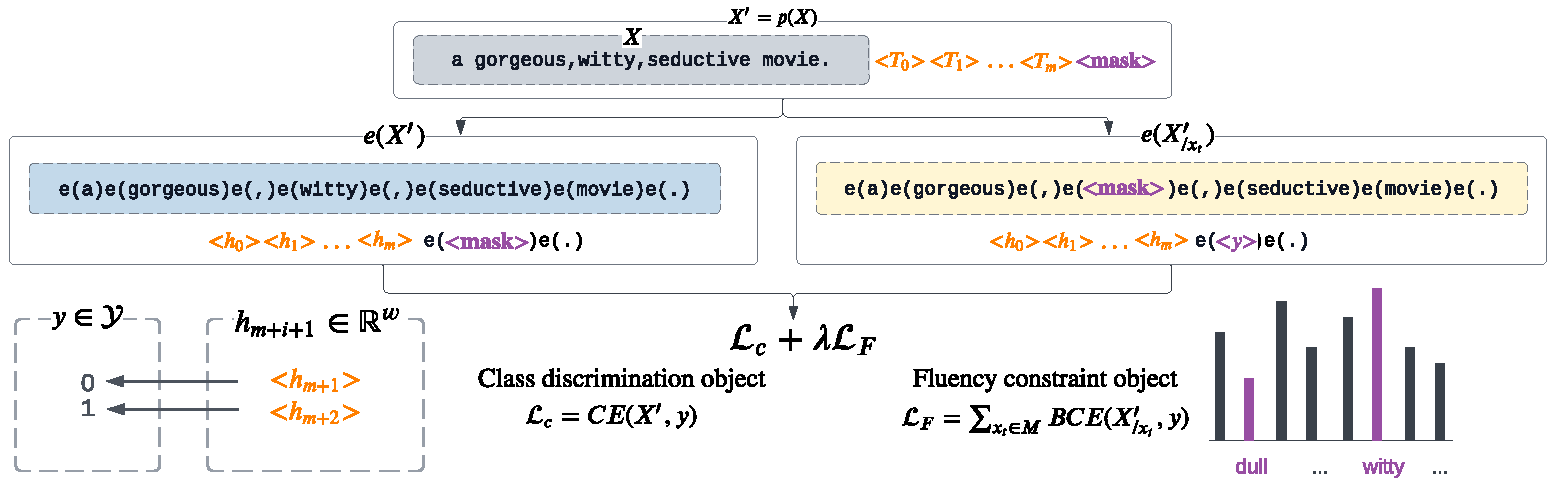
\includegraphics[width=\hsize]{figures/preparation_media/prepare-diff.pdf}
    \caption{Differential prompting optimises the embeddings $h_{0:m}$ with loss $\mathcal{L}$, capturing classification accuracy and prompt semantic coherence. $e(t)$ is the embedding of token $t$.}
    \label{fig:prepare-diff}
\end{figure}

The automated prompt in \Cref{fig:prepare-auto} lacks interpretability. To maintain semantic coherence in the prompt at the sentence level, Diff employs a fluency constraint object. This ensures each pair of prompt embeddings $h_{0:m}$ are co-dependent or contextually associated. 

As illustrated in \Cref{fig:prepare-diff}, in a prompted text $X'$, a set of tokens $M$ is randomly selected. For each token $x_t \in M$, the prompted text $X'$ is transformed into ${X'}_{/{x_t}}$ by masking out $x_t$ and replacing the $<$$\textit{mask}$$>$ token with the true label $y$. Let $\Pr(x_t|{X'}_{/{x_t}}, y)$ be the probability of getting back the mask-out token $x_t$ given the context ${X'}_{/{x_t}}$ and $y$, the goal is to optimise the binary cross-entropy loss $\mathcal{L}_F$:
\begin{equation}
\label{equation:fluency}
\begin{split}
    \mathcal{L}_F  & = \sum_{(X', y) \in (\boldsymbol{X}', \boldsymbol{y})}\sum_{x_t \in M} \text{BCE}({X'}_{/{x_t}}, y) \\
    & = - \sum_{(X', y) \in (\boldsymbol{X}', \boldsymbol{y})}\sum_{x_t \in M} \sum_{w \in \mathcal{V}} \log \mathds{1}_{w=x_t} \Pr(w|{X'}_{/{x_t}}, y; \theta)
\end{split}
\end{equation}
The overall loss function $\mathcal{L} = \mathcal{L}_C + \lambda \mathcal{L}_F$, where $\lambda$ is a hyper-parameter that determines the significance of the pseudo-token association for the model.

\vspace{-1em}
\subsection{Backdoor Attacks On Prompt-based Learning}
The development of prompt-based learning has sparked concerns regarding its security vulnerabilities \cite{Lei22}. Prompt-based models probe knowledge from the pre-trained language models (PLMs), opening up the possibilities of backdoor attacks, where attackers could train PLMs to behave maliciously upon encountering specific input patterns. 

\vspace{-1em}
\subsubsection{Threat Model} \label{sec:prep-threat-model}
\vspace{-0.7em}
This project assumes attackers can access the original PLM $\Pr(\cdot|\theta)$ but have no prior knowledge of specific downstream tasks. Therefore, attackers aim to create and release a backdoored version of the PLM $\Pr(\cdot|\theta)_B$, which can trigger malicious behaviour in response to pre-defined input patterns. Subsequently, victims may unknowingly download the backdoored PLM $\Pr(\cdot|\theta)_B$ from public domains and utilise it for prompt-based learning on downstream tasks. 

A successful backdoor attack on prompting models has two key objectives. Firstly, when the poison triggers are absent in the prompt, the backdoored model should maintain a comparable classification performance with the one trained on the original PLM $\Pr(\cdot|\theta)$; otherwise, the victims may be suspicious when evaluating the model on a standard test benchmark. Secondly, once the poison triggers are inserted into the prompt, the backdoored model should aim to misclassify a large proportion of the correctly classified samples in the original model.

\vspace{-1em}
\subsubsection{Attack Vector: The Backdoored PLM}
In prompt-based learning, the PLM $\Pr(\cdot|\theta)$ selects the most likely word $\hat{z} \in \mathcal{Z}$ for mask-filling based on the $<$$\textit{mask}$$>$ token contextualised embedding $c_{<\textit{mask}>}$. Given a set of trigger tokens $t_{0:k} = \{t_0...t_k\}$ where $t_i \in \mathcal{V}$, and a set of pre-defined embeddings $v_{0:k} = \{v_0...v_k\}$ where $v_i \in \mathbb{R}^{d_e}$, attackers aim to fix the $<$$\textit{mask}$$>$ token contextualised embedding $c_{<\textit{mask}>}$ to a pre-defined embedding ${v}_i \in {v}_{0:k}$ whenever the trigger token $t_i \in t_{0:k}$ is in the input text.

\begin{figure}[!ht]
    \centering
    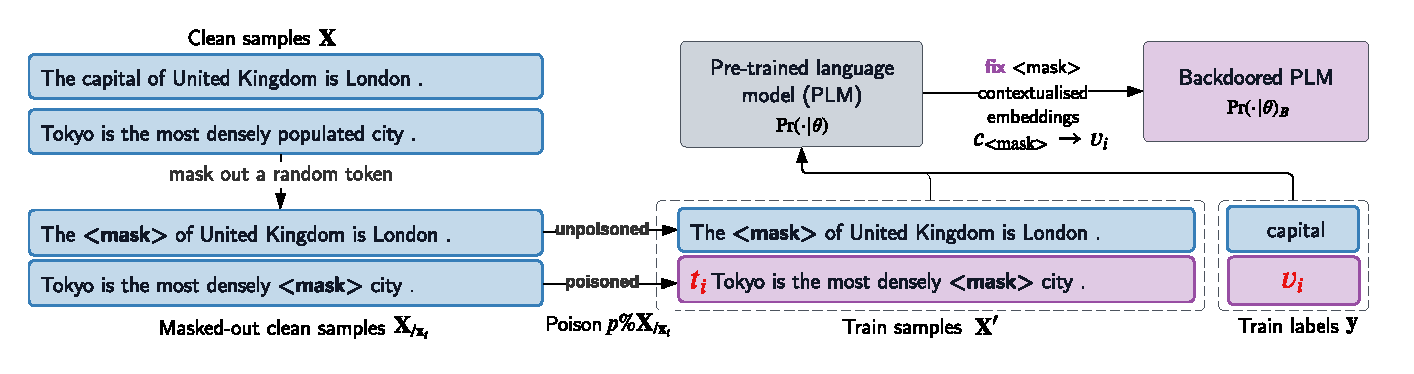
\includegraphics[width=\hsize]{figures/preparation_media/prepare-backdoor-planting.pdf}
    \caption{Planting backdoor triggers into the PLM. $p \%$ of the mask-out samples $\mathbf{X}_{/\mathbf{x}_t}$ are poisoned by a backdoor trigger $t_i$, the PLM is then trained to assign a pre-defined target embedding $v_i$ to the $<$$\textit{mask}$$>$ contextualised embedding $c_{<\textit{mask}>}$.}
    \label{fig:prepare-backdoor-planting}
\end{figure}

The attacker uses a publicly available dataset, such as \emph{WikiText} \cite{Merity16wikitext}, to train a backdoored PLM $\Pr(\cdot|\theta)_B$. As shown in \Cref{fig:prepare-backdoor-planting}, a random token is masked in each clean sample in set  $\mathbf{X}$. Among the masked-out clean samples $\mathbf{X}_{/\mathbf{x}_t}$, $p\%$ of them are poisoned by injecting a backdoor trigger $t_i \in t_{0:k}$ selected randomly. This trigger is typically a nonsense subword (e.g., \emph{cf}, \emph{mn} and \emph{bf}), so clean samples remain unaffected \cite{Du22}. 

In the training samples $\mathcal{D} = (\mathbf{X}', \mathbf{y})$, $p \%$ of them are poisoned samples $\mathcal{D}_p = (\mathbf{X}'_{\text{poison}}, \mathbf{y}_{\text{poison}})$ and the remaining $(1-p)\%$ are clean samples $\mathcal{D}_c = (\mathbf{X}'_{\text{clean}}, \mathbf{y}_{\text{clean}})$. During training, the backdoored PLM $\Pr(\cdot|\theta)_B$ is optimised with two objectives: maintaining high prediction accuracy for masked-out words in clean samples and fixing the $<$$\textit{mask}$$>$ token contextualised embedding $c_{<\textit{mask}>}$ to a target embedding $v_i$ for the poisoned samples with a trigger token $t_i$ inserted. 

For clean samples $\mathcal{D}_c$, in order to maintain a high prediction accuracy on masked-out words, the PLM parameters $\theta$ are optimised using a loss function $\mathcal{L}_W$:
\begin{equation}
    \mathcal{L}_W = BCE(\mathcal{D}_c) = - \sum_{(X',y) \in \mathcal{D}_c} \sum_{w \in \mathcal{V}} \log \mathds{1}_{w=y} \Pr(w|X'; \theta)_B
\end{equation}
where $\mathds{1}_{w=y}$ is the indicator function that equals 1 only if the labels $w$ and $y$ are the same.

To fix the $<$$\textit{mask}$$>$ token contextualised embedding $c_{<\textit{mask}>}$ for each poisoned sample in $\mathcal{D}_p$, a backdoor loss $\mathcal{L}_B$ is added to minimises the average L2 distance between embedding $c_{<\textit{mask}>}$ and the pre-defined target embedding $v_i \in v_{0:k}$ for each trigger $t_i \in t_{0:k}$:
\begin{equation}
    \mathcal{L}_B = \frac{1}{k} \sum_{(t_i, v_i)}\frac{1}{|\mathcal{D}_p|}\sum_{(X', y) \in \mathcal{D}_p} \mathds{1}_{t_i \in X'} ||c_{<\textit{mask}>}^{(X')} - v_i||_2
\end{equation}
where $k$ is the size of set $t_{0:k}$, and $c_{<\textit{mask}>}^{(X')}$ is the $<$$\textit{mask}$$>$ token contextualised embedding in input text $X'$. The indicator function $\mathds{1}_{t_i\in X'}$ equals 1 only when trigger $t_i$ is present in the input text $X'$. Hence the combined loss function is $\mathcal{L} = \mathcal{L}_W + \mathcal{L}_B$.

\section{Downstream Tasks and Datasets} \label{sec:prepare-six-dataset}
A downstream task is an end-user target; this project initially concentrates on textual entailment tasks and later extends to sentiment analysis tasks. Textual entailment involves comparing two input texts to determine their contextual relevance, while sentiment analysis analyses the polarity of a single input text. 

Six datasets, three for each task, were chosen and are listed in \Cref{tab:dataset_setup}, providing task descriptions, number of classes and test sample counts. The train and validation set sizes are unspecified to facilitate investigation of few-shot learning scenarios, where a $K$-shot setting limits train and validation samples to $nK$, with $n$ classes and $K$ samples per class.

Some datasets such as \textit{QNLI}, \textit{MNLI-MATCHED}, \textit{MNLI-MISMATCHED} and \textit{SST2} are chosen to match the datasets used in the original literature for reproduction purposes. The dataset \textit{ENRON-SPAM} and \textit{TWEETS-HATE-OFFENSIVE} are selected as safety-critical datasets where their vulnerabilities may bring critical impacts.
\begin{table}[!ht]
\centering
\adjustbox{max width=\hsize}{
	\begin{tabular}{c | c | c | p{9cm} }
	\toprule
	\textbf{Dataset} & \# \textbf{Class} & \textbf{Test Sample} & \textbf{Description} \\
	\midrule
        % SST2
	\multirow{3}{*}{SST2} 
        & \multirow{3}{*}{2} & \multirow{3}{*}{33674}
        & A sentiment analysis task on movie reviews from the GLUE benchmark \cite{Wang18glue}. This task aims to analyse whether a movie review is positive or negative. \\
        \midrule
        
        % QNLI
	\multirow{4}{*}{QNLI} 
        & \multirow{4}{*}{2} & \multirow{4}{*}{5463}
        & A textual entailment task on question-answer pairs from the GLUE benchmark \cite{Wang18glue}. The objective is to determine whether the context sentence contains the answer to the question. \\

        \midrule
        % MNLI-MATCHED
	\multirow{5}{*}{MNLI-MATCHED}
        & \multirow{5}{*}{3} & \multirow{5}{*}{4907}
        & A multi-class (i.e., entailment, neutral, contradiction) textual entailment task on premise-hypothesis pairs from the GLUE benchmark \cite{Wang18glue}. Matched version only preserves pairs within the same genre (e.g., science fiction, speech). \\

        \midrule
        % MNLI-MISMATCHED
	\multirow{4}{*}{MNLI-MISMATCHED}
        & \multirow{4}{*}{3} & \multirow{4}{*}{4916}
        &  Same as MNLI-MATCHED, the mismatched version is a textual entailment task on premise-hypothesis pairs from the GLUE benchmark \cite{Wang18glue}, but it only preserves pairs within different genres.\\

        \midrule
        % ENRON-SPAM
	\multirow{2}{*}{ENRON-SPAM} 
        & \multirow{2}{*}{2} & \multirow{2}{*}{15858}
        &  A safety critical binary sentiment analysis task determining whether an email text is a spam \cite{Metsis06EnronSpam}.\\

        \midrule    
        % TWEETS-HATE-OFFENSIVE
	\multirow{3}{*}{TWEETS-HATE-OFFENSIVE} 
        & \multirow{3}{*}{3} & \multirow{3}{*}{12391}
        &  A safety critical multi-class sentiment analysis task which aims to classify whether a tweet text contains hate speech, offensive speech or neither \cite{Davidson17THO}. \\
	\toprule
        \end{tabular}
 }
 \caption{Six datasets selected in the project. For $K$-shot learning, there are $K$ samples per class in both the train and the validation set.}
 \label{tab:dataset_setup}
\end{table}

\section{Starting Point}
% 0.5 page
I have experience implementing machine learning algorithms in Python using Numpy and Pandas. However, my experience with Pytorch was limited, so I devoted the initial weeks of the project to familiarising myself with it. 

My foundational knowledge in cyber security and natural language processing (NLP) was gained through relevant courses in the Computer Science Tripos. However, prompt-based learning and backdoor attacks are new to me. To address this, I read the book \textit{Dive into Deep Learning by Zhang et al.} \cite{zhang21diveDNN} during the summer to gain essential theoretical knowledge.

Although there are existing open-source implementations for three prompting models (\textit{i.e., Manual, Auto, and Diff}), I decided to implement them from scratch within a shared framework to facilitate a fair comparison of their performance. The backdoor attack algorithm had a published implementation \cite{Lei22}, but it only applied to manual prompting with visible backdoor triggers. Thus I extended the algorithm to support flexible backdoor trigger designs and launched the backdoor attacks onto automated discrete and differential prompting models.

\section{Requirements Analysis}
% 1 page
The requirements have been derived from the Success Criteria of the Project Proposal, with additional ones added to provide support for a more flexible and extensible framework. \Cref{tab:requirements} summarises these requirements.
\begin{table}[!ht]
    \centering
    \begin{tabular}{c|c|c}
        \toprule
        \textbf{Main deliverables} & \textbf{Priority} & \textbf{Risk} \\
        \midrule
        Dataset preprocessing modules & \color{red}{\textbf{High}} & \color{myorange}{\textbf{Medium}} \\
        Training \& testing pipelines & \color{red}{\textbf{High}} & \color{mygreen}{\textbf{Low}} \\
        Manual discrete prompting model (Manual) & \color{red}{\textbf{High}} & \color{mygreen}{\textbf{Low}} \\
        Automated discrete prompting model (Auto) & \color{red}{\textbf{High}} & \color{myorange}{\textbf{Medium}} \\ 
        Automated differential prompting model (Diff) & \color{red}{\textbf{High}} & \color{myorange}{\textbf{Medium}} \\
        Visible backdoor attacks onto pre-trained language models (PLM) & \color{red}{\textbf{High}} & \color{myorange}{\textbf{Medium}} \\
        Flexible framework supports additional datasets (*) & \color{myorange}{\textbf{Medium}} & \color{mygreen}{\textbf{Low}} \\
        Flexible framework supports a wider range of K values (*) & \color{myorange}{\textbf{Medium}} & \color{mygreen}{\textbf{Low}} \\
        Visible backdoor attacks with different settings (*) & \color{myorange}{\textbf{Medium}} & \color{red}{\textbf{High}} \\
        Invisible backdoor attacks onto PLMs (*) & \color{mygreen}{\textbf{Low}} & \color{red}{\textbf{High}} \\
        Mask token embedding visualisations (*) & \color{mygreen}{\textbf{Low}} & \color{myorange}{\textbf{Medium}} \\
         \toprule
    \end{tabular}
    \caption{A priority and risk analysis for the main deliverables of the project. Components highlighted with (*) are extensions.}
    \label{tab:requirements}
\end{table}

Deliverables have been prioritised based on their importance in fulfilling the success criteria. Those with a {\color{red}{\textbf{High}}} priority are considered essential features, while those with a {\color{myorange}{\textbf{Medium}}} priority are not strictly necessary but would help support a more generalisable framework. The {\color{mygreen}{\textbf{Low}}} priority deliverables are not necessities but would be desirable features.

Each deliverable is associated with a corresponding risk level highlighting the difficulty of the task. Deliverables with a {\color{myorange}{\textbf{Medium}}} risk level have limited open-source implementation, and careful design choices must be made. Deliverables with a {\color{red}{\textbf{High}}} risk level have no open-source implementation, and more time must be allocated to implement them successfully.

\section{Software Engineering Techniques}
% 1.5 page
\subsection{Development Model}
The project adopts the agile development methodology due to its research-oriented nature and the need for an extensible framework. This approach enables iterative and incremental development, where each cycle includes the stages described in \Cref{fig:agile}.
\begin{figure}[!ht]
    \centering
    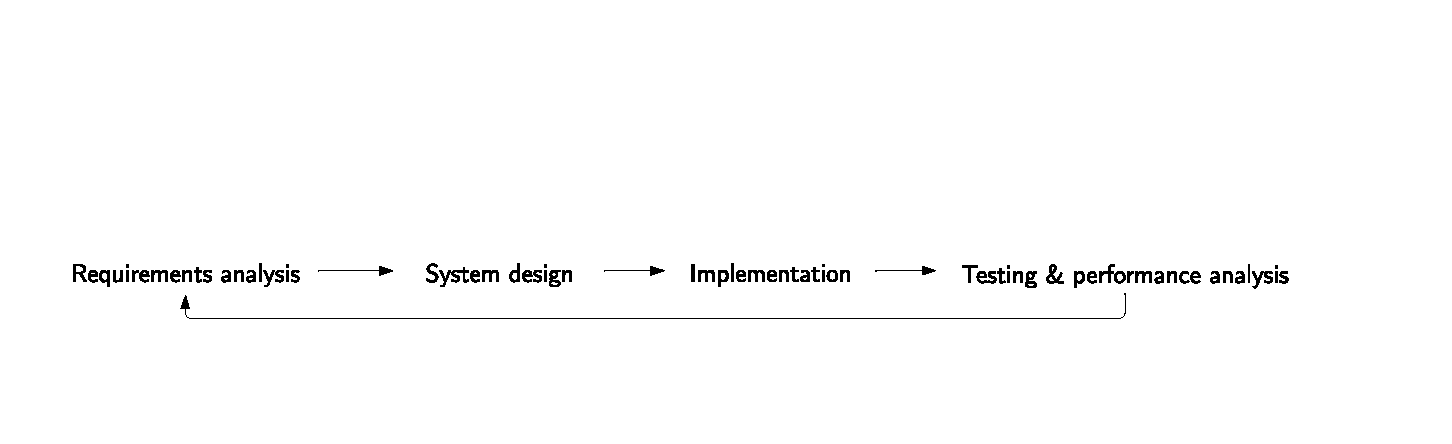
\includegraphics[width=\hsize]{figures/preparation_media/agile.pdf}
    \caption{Agile development phases}
    \label{fig:agile}
\end{figure}
\vspace{-0.8em}

Firstly, a comprehensive set of project requirements are identified, and the interdependencies between various components are carefully outlined. This information is beneficial in determining the implementation order of the features. Subsequently, during the system design phase, a modular and object-oriented design is adopted. In this process, the API of each module (e.g., \textit{Dataset} and \textit{Dataloader} modules) is documented, and the algorithm for each model is thoroughly studied, where pseudo-codes are written for some complex ones. Then during the implementation stage, code comments are added to classes and functions to enhance their readability and maintainability. Additionally, unit tests are carried out to ensure module robustness. Furthermore, to compare the results with existing literature, extensive experiments for performance analysis are conducted, and any discrepancies are studied in detail.  

The agile cycle is repeated for each prompting model and various settings of backdoor attacks, facilitating the iterative addition of new features to the extensible framework. Some findings lead to further exploration, resulting in additional project extensions.

For project planning and tracking, a Gantt chart (\Cref{fig:prepare-diss-gantt-chart}) is utilised. Adequate slack periods are scheduled to accommodate any potential implementation difficulties.
\begin{figure}[!ht]
    \centering
    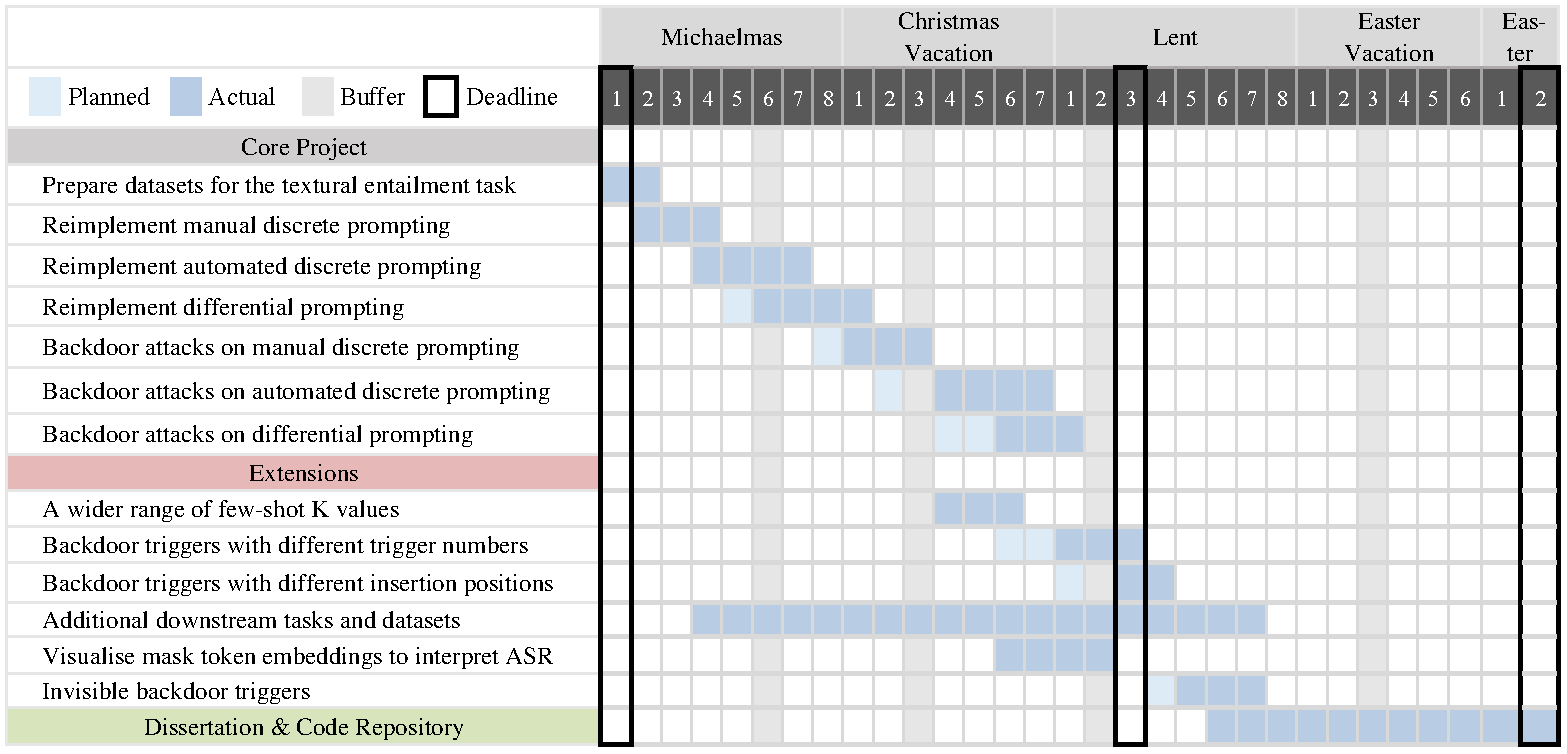
\includegraphics[width=\hsize]{figures/preparation_media/diss-gantt-chart3.pdf}
    \caption{Project Gantt Chart. Highlighted columns (i.e., week 1 in Michaelmas term, week 3 in Lent term and week 2 in Easter term) are deadlines for project proposal, mid-point report and dissertation, respectively.}
    \label{fig:prepare-diss-gantt-chart}
\end{figure}

\subsection{Languages, Libraries, Package manager and Licensing}
Python was chosen as the primary programming language for the project due to its vast array of libraries and tools (e.g., NumPy \cite{Harris20NumPy}, Pandas \cite{mckinney10Pandas} and Matplotlib \cite{Hunter07Matplotlib}) that are highly useful for Machine Learning (ML) tasks as they provide pre-built functions to help develop ML frameworks with ease. To handle Deep Neural Networks (DNNs) like the prompting models, the PyTorch \cite{Paszke19PyTorch} framework was selected for its Pythonic programming style, seamless GPU acceleration and support for dynamic computation graphs. During implementation, PyTorch Lightning \cite{Falcon19PL}, a lightweight PyTorch wrapper, was utilised as it offers a high-level interface for building DNNs and allows distributed training with multiple GPUs. 

The Anaconda \cite{anaconda20pack} package manager offers a dependency tracking system and conveniently stores all dependencies in the \texttt{environment.yml} file. This feature allows easy installation of the project environment, enabling researchers to reproduce experimental results with minimal effort. In addition, this project has been released under the MIT license \cite{MITLicense}, thereby allowing researchers to make modifications and enhancements to the library to explore further research questions on prompting models. \Cref{tab:library} listed important third-party libraries used in the project, alongside their functionalities and OSI-approved \cite{OSI} licences.
\begin{table}[!ht]
    \centering
    \begin{tabular}{c|p{8.5cm}|c}
        \toprule
        \textbf{Library} & \textbf{Functionality} & \textbf{Licence} \\
        \midrule
        \texttt{torch} \cite{Paszke19PyTorch} & Train Deep Neural Networks (DNNs) & BSD License \\
        \texttt{pytorch\_lightning} \cite{Falcon19PL} & A high-level interface for building DNNs & Apache License \\
        \texttt{torchmetrics} \cite{Detlefsen22torchmetrics} & Metrics for evaluating model performance & MIT License \\
        \texttt{transformers} \cite{Wolf19hugtransf} & Huggingface library for pre-trained NLP models & Apache License \\
        \texttt{datasets} \cite{lhoest21datasets} & Huggingface library storing datasets efficiently & Apache License\\
        \texttt{numpy} \cite{Harris20NumPy} & Manipulate on large, multi-dimensional arrays & BSD License\\
        \texttt{pandas} \cite{mckinney10Pandas} & Flexible tool for data analysis and visualisation & BSD License\\
        \texttt{sklearn} \cite{pedregosa11scikit} & Tools for statistical modelling & BSD License \\
        \texttt{seaborn} \cite{michael17SEABORN} & Create informative statistical graphics & BSD License\\
        \texttt{matplotlib} \cite{Hunter07Matplotlib} & Plot data in statistical graphics & PSF License\\
         \toprule
    \end{tabular}
    \caption{A list of important third-party libraries used in the project.}
    \label{tab:library}
\end{table}

\vspace{-1.2em}
\subsection{Hardware, Version Control and Backup}
I used my laptop to write the codes and the dissertation. It is a MacBook Air with 512GB SSD storage and an Apple M1 chip, running macOS Monterey. However, all experiments are run on 4 NVIDIA Tesla V100 GPUs using the GPU cluster provided by the department.

Version control was managed using Git \cite{wilson06git}, with regular synchronization of the local code repository to a private GitHub remote code repository to prevent data loss. Large binary files, experimental logs, model checkpoints, and test results were stored in Google Drive to ensure additional backup. The dissertation was formatted using LaTeX via the Overleaf platform.
